\section{Numerical Experiments}

\subsection{Implementation of the algorithms}

We use Python to compare full pivoting cross approximation (fpCA), partial pivoting cross approximation (ppCA), and an adaptive version of ppCA. The implementation separates the computation of the low-rank factors from the computation of the error curves. The functions \texttt{fpCA\_approx} and \texttt{ppCA\_approx} return only the two factor matrices $U$ and $V$, while the error-analysis routines compute the relative Frobenius errors afterwards. This makes it possible to measure separately the time spent constructing the approximation and the time spent evaluating the error.

For a matrix $A \in \mathbb{R}^{m \times n}$ and a rank-$k$ approximation
\[
  \widehat{A}_k = \sum_{\mu=1}^{k} u_\mu v_\mu^T,
\]
we measure the error by the relative Frobenius norm
\[
  e_k = \frac{\|A - \widehat{A}_k\|_F}{\|A\|_F}.
\]
The error is plotted against the rank $k$ on a logarithmic scale. The singular value decomposition (SVD) is included as a reference curve, since it gives the best rank-$k$ approximation in the Frobenius norm.

The numerical experiments in the code use maximum rank $150$ for the matrix-based experiments. The Iris kernel matrices have size $150 \times 150$. The synthetic matrices and the California housing kernel matrix are tested with size $1000 \times 1000$. A separate matrix-free ppCA experiment is also included for the Iris Gaussian kernel, using only entry evaluations of the kernel function.

\subsubsection*{Full pivoting cross approximation}

In full pivoting, the pivot is chosen as the largest entry of the current residual matrix. This gives a stable pivot choice, but it requires searching the whole residual matrix at every step. For a dense $n \times n$ matrix, this search costs $O(n^2)$ per iteration and the method also stores and updates the full residual matrix.

\begin{algorithmic}[1]
    \Require Matrix $A$, maximum rank $k_{\max}$, tolerance $\varepsilon$
    \State $R = A$
    \For{$k = 1,\ldots,k_{\max}$}
        \State $(i_k,j_k) = \arg\max_{i,j} |R_{ij}|$
        \State $p = R_{i_k j_k}$
        \If{$|p| < \varepsilon$}
            \State stop
        \EndIf
        \State $u_k = R(:,j_k)$
        \State $v_k = R(i_k,:)/p$
        \State $R = R - u_k v_k^T$
    \EndFor
\end{algorithmic}

In the code, the actual rank can be smaller than $k_{\max}$ if the pivot falls below the tolerance. The routine returns the truncated factors $U$ and $V$.

\subsubsection*{Partial pivoting cross approximation}

In partial pivoting, the method does not search over the whole residual. Instead, it starts from a pivot row, chooses the largest entry in that residual row as the pivot column, computes the corresponding residual column, and then chooses the next pivot row from this column. Thus each iteration uses one row and one column rather than the entire residual matrix.

\begin{algorithmic}[1]
    \Require Matrix $A$, maximum rank $k_{\max}$, tolerance $\varepsilon$
    \State Choose an initial pivot row $i_1$
    \For{$k = 1,\ldots,k_{\max}$}
        \State Compute the residual row $b = R(i_k,:)$
        \State $j_k = \arg\max_j |b_j|$
        \State $p = b_{j_k}$
        \If{$|p| < \varepsilon$}
            \State stop
        \EndIf
        \State Compute the residual column $a = R(:,j_k)$
        \State $u_k = a/p$
        \State $v_k = b$
        \State Choose the next pivot row from $|u_k|$, ignoring the current row
    \EndFor
\end{algorithmic}

The implementation avoids immediately choosing the same pivot row again by setting the current row entry to zero before taking the next maximum:
\[
  w = |u_k|, \qquad w_{i_k}=0, \qquad i_{k+1}=\arg\max_i w_i .
\]

\subsubsection*{Adaptive partial pivoting}

The adaptive ppCA routine uses the same pivoting strategy, but also has a stopping rule based on the size of the new rank-one update. If $u_k$ and $v_k$ are the vectors in the current update, the algorithm stops when
\[
  \|u_k\|_2 \|v_k\|_2
  \leq
  \varepsilon \|u_1\|_2 \|v_1\|_2 .
\]
In the present code, the adaptive routine returns the relative Frobenius error after each accepted update. Therefore, unlike \texttt{fpCA\_approx} and \texttt{ppCA\_approx}, it is used directly as an error-producing routine in the plots.

\subsection{Test matrices and data sets}

\subsubsection*{Synthetic matrices}

The synthetic matrices are generated with size $n=1000$. The first two have the form
\[
  A = U \Sigma V^T,
\]
where $U$ and $V$ are random orthogonal matrices obtained from QR decompositions. The diagonal matrix $\Sigma$ controls the singular value decay.

For the first matrix, the singular values decay exponentially after $R=5$ dominant values:
\[
  \sigma_k =
  \begin{cases}
    1, & k \leq R, \\
    10^{-(k-R)q}, & k > R,
  \end{cases}
  \qquad q = 0.15 .
\]
This matrix is close to low rank because the singular values decrease quickly.

For the second matrix, the singular values decay polynomially after $R=15$ dominant values:
\[
  \sigma_k =
  \begin{cases}
    1, & k \leq R, \\
    (k-R+1)^{-p}, & k > R,
  \end{cases}
  \qquad p = 1.8 .
\]
This is harder to approximate because the tail decays more slowly.

The third synthetic matrix is a low-rank positive semidefinite signal with positive semidefinite noise,
\[
  A_3 = A_{\mathrm{signal}} + \xi W,
\]
where $A_{\mathrm{signal}}$ has $R=10$ dominant diagonal entries, $\xi=0.5$, and $W = GG^T/n$ with $G$ a random Gaussian matrix.

\subsubsection*{Kernel matrices}

The code also tests kernel matrices from real data. For the Iris data set, both a Gaussian kernel and a linear kernel are used. The Iris data set has $150$ samples, so these matrices are $150 \times 150$.

The linear kernel is
\[
  K_{ij} = x_i^T x_j .
\]
The Gaussian kernel matrix routine uses
\[
  K_{ij}
  =
  \exp\!\left(-\frac{\|x_i-x_j\|_2^2}{2\sigma^2}\right),
  \qquad \sigma = 1 .
\]
The California housing experiment uses the first $1000$ samples of the data set and forms the corresponding $1000 \times 1000$ Gaussian kernel matrix.

\subsubsection*{Matrix-free kernel experiment}

The final experiment uses a function interface for ppCA. Instead of forming a matrix in advance, the entries are computed by a function $K(i,j)$ whenever they are needed. This experiment is performed on the Iris Gaussian kernel with maximum rank $10$. The error is still computed by looping over all entries, so the test is matrix-free for the approximation step but not for the error evaluation.

\subsection{Output of the experiment script}

The updated Python script saves every figure as a PDF file in a directory called \texttt{plots}. It no longer calls \texttt{plt.show()} for the final output. The generated figure files are:
\[
\begin{array}{ll}
\texttt{iris\_gaussian\_kernel.pdf}, & \text{Iris Gaussian kernel}, \\
\texttt{iris\_linear\_kernel.pdf}, & \text{Iris linear kernel}, \\
\texttt{synthetic\_A1.pdf}, & \text{synthetic exponential decay matrix}, \\
\texttt{synthetic\_A2.pdf}, & \text{synthetic polynomial decay matrix}, \\
\texttt{synthetic\_A3.pdf}, & \text{synthetic low-rank matrix with PSD noise}, \\
\texttt{california\_gaussian\_kernel.pdf}, & \text{California housing Gaussian kernel}, \\
\texttt{matrix\_free\_iris\_gaussian\_kernel.pdf}, & \text{matrix-free Iris Gaussian kernel experiment}.
\end{array}
\]

\subsection{Results}

\subsubsection*{Iris kernel matrices}

Figure~\ref{fig:iris_gaussian_kernel} shows the approximation error for the Iris Gaussian kernel matrix. The SVD curve is the reference best possible error. Full pivoting is generally expected to be more stable than partial pivoting because it searches the full residual, while ppCA and adaptive ppCA use only local row and column information.

\begin{figure}[h]
    \centering
    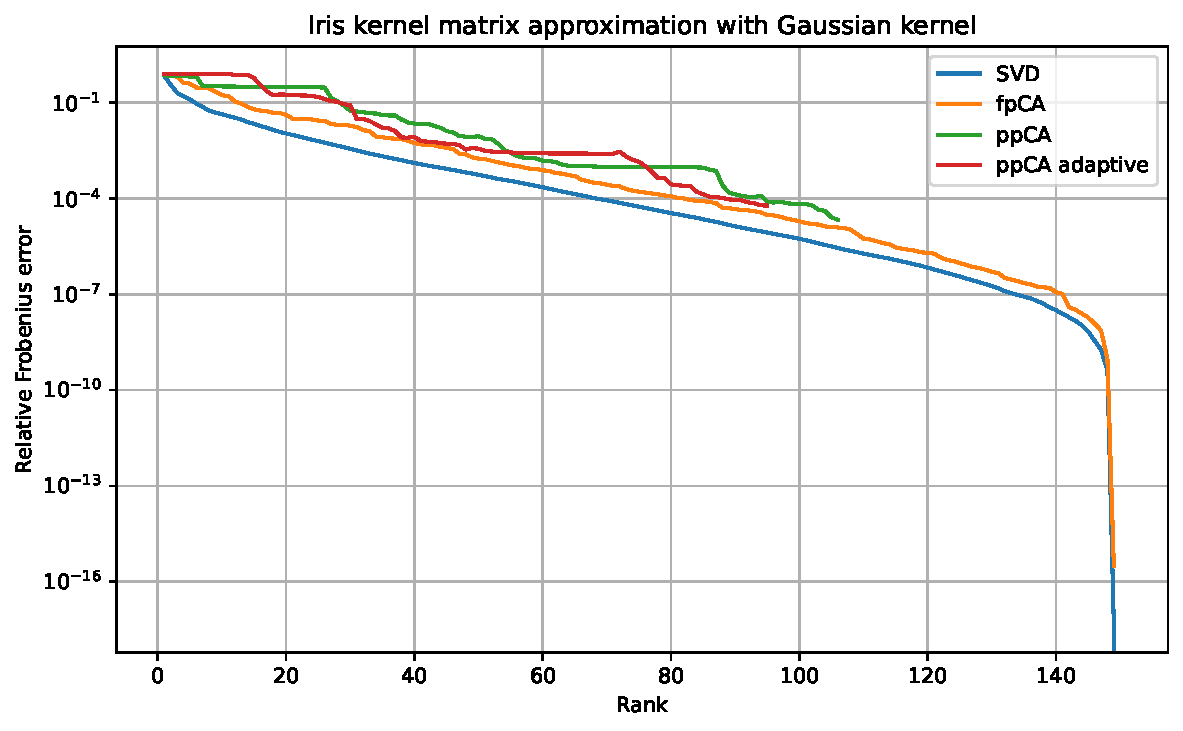
\includegraphics[width=0.85\textwidth]{plots/iris_gaussian_kernel.pdf}
    \caption{Relative Frobenius error for the Iris Gaussian kernel matrix.}
    \label{fig:iris_gaussian_kernel}
\end{figure}

Figure~\ref{fig:iris_linear_kernel} shows the result for the Iris linear kernel. Since the Iris data have only four features, the linear kernel matrix has rank at most four. Therefore, the approximation error should drop after only a few rank-one updates.

\begin{figure}[h]
    \centering
    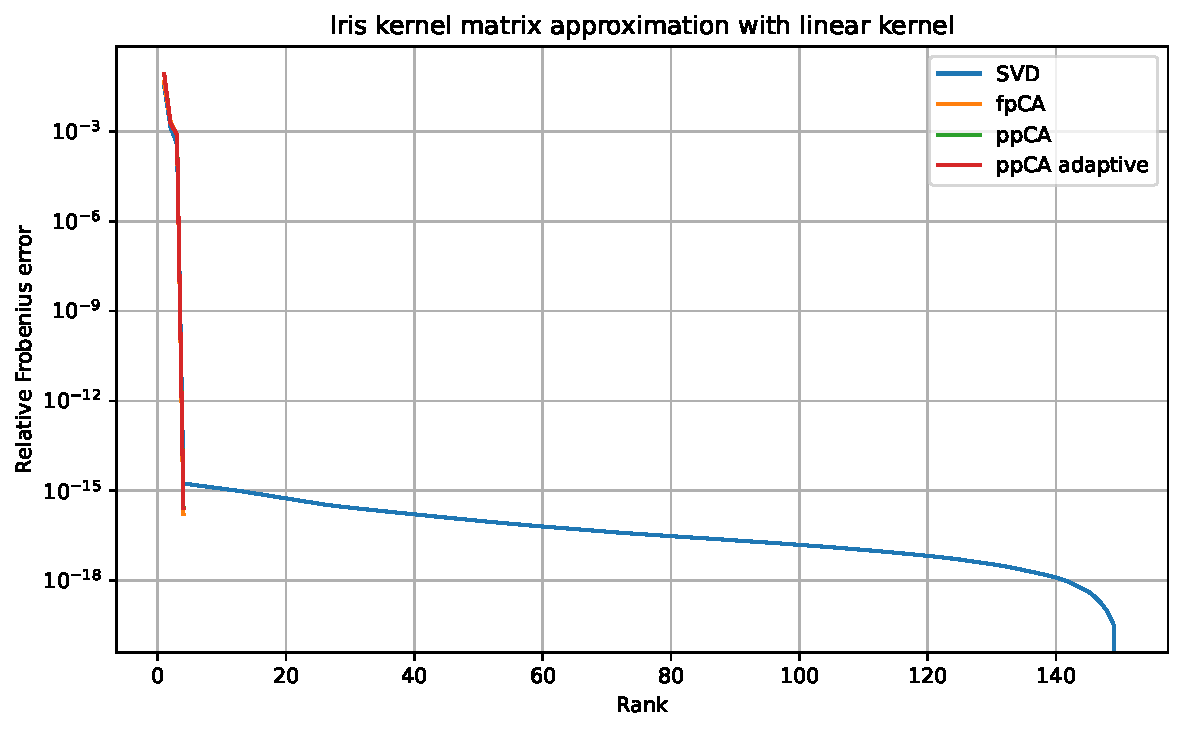
\includegraphics[width=0.85\textwidth]{plots/iris_linear_kernel.pdf}
    \caption{Relative Frobenius error for the Iris linear kernel matrix.}
    \label{fig:iris_linear_kernel}
\end{figure}

\subsubsection*{Synthetic matrices}

Figure~\ref{fig:synthetic_A1} shows the synthetic matrix with exponential singular value decay. The fast decay means that a small rank already captures most of the matrix energy.

\begin{figure}[h]
    \centering
    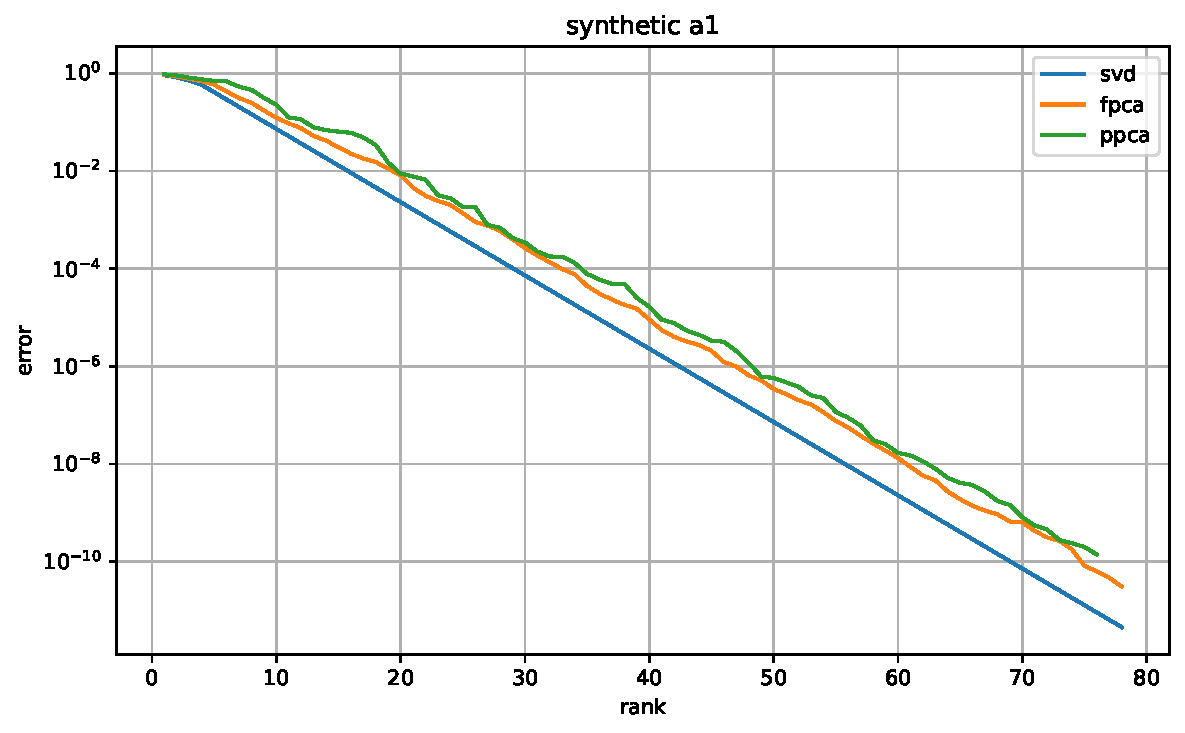
\includegraphics[width=0.85\textwidth]{plots/synthetic_A1.pdf}
    \caption{Relative Frobenius error for synthetic matrix A1 with exponential singular value decay.}
    \label{fig:synthetic_A1}
\end{figure}

Figure~\ref{fig:synthetic_A2} shows the polynomial decay matrix. The error decreases more slowly because the singular values have a heavier tail.

\begin{figure}[h]
    \centering
    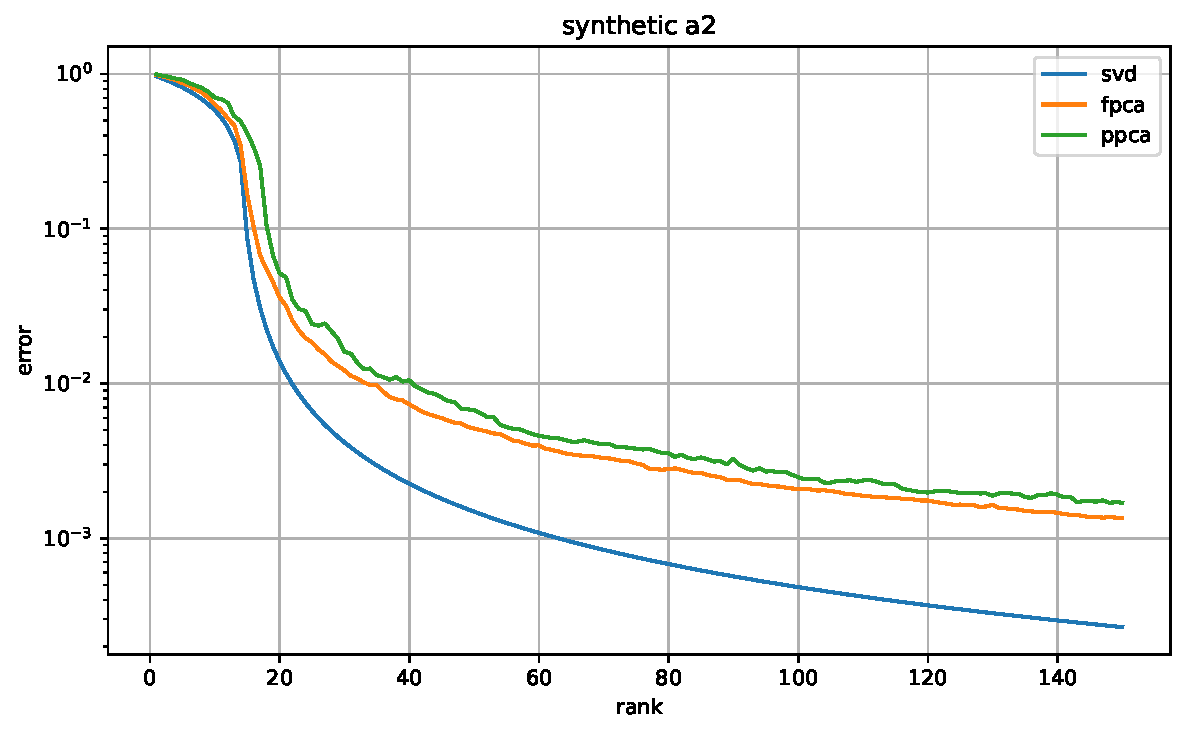
\includegraphics[width=0.85\textwidth]{plots/synthetic_A2.pdf}
    \caption{Relative Frobenius error for synthetic matrix A2 with polynomial singular value decay.}
    \label{fig:synthetic_A2}
\end{figure}

Figure~\ref{fig:synthetic_A3} shows the low-rank positive semidefinite matrix with noise. The added noise spreads energy over many directions, so more rank is needed than for a clean low-rank matrix.

\begin{figure}[h]
    \centering
    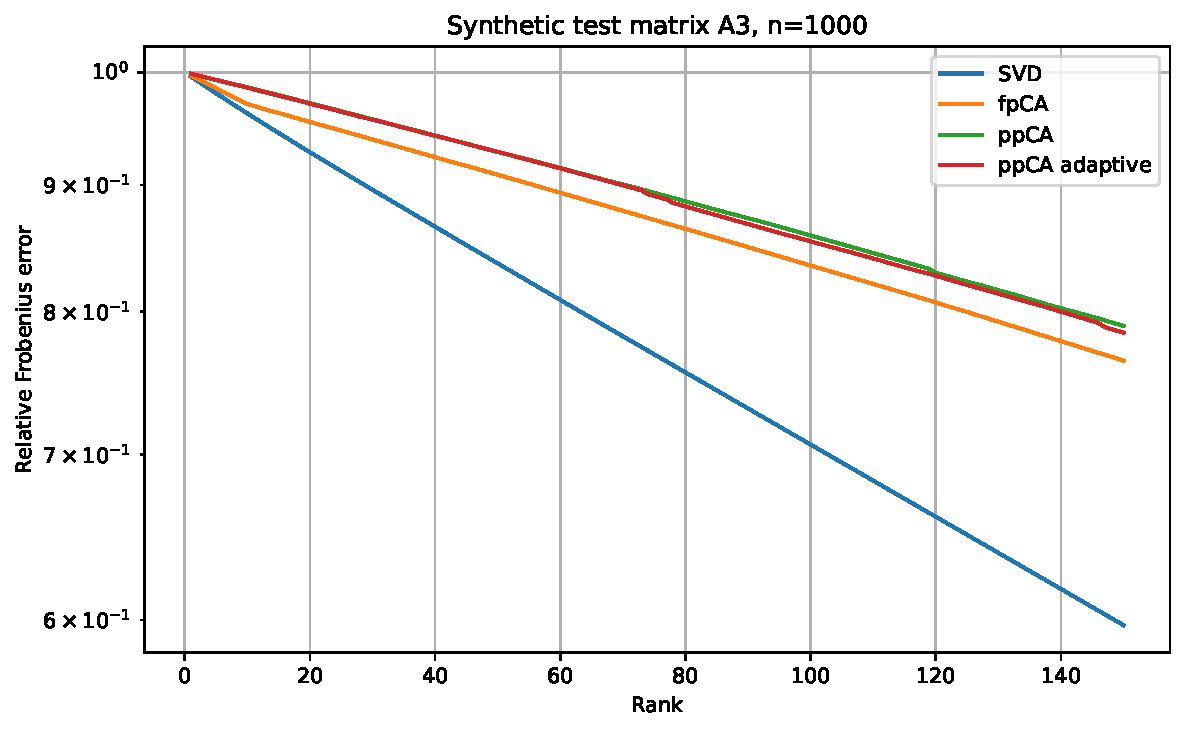
\includegraphics[width=0.85\textwidth]{plots/synthetic_A3.pdf}
    \caption{Relative Frobenius error for synthetic matrix A3, a low-rank PSD signal with PSD noise.}
    \label{fig:synthetic_A3}
\end{figure}

\subsubsection*{California housing kernel matrix}

Figure~\ref{fig:california_gaussian_kernel} shows the Gaussian kernel matrix formed from the first $1000$ California housing samples. This experiment is larger than the Iris experiments and is included to test the behavior on a more realistic dense kernel matrix.

\begin{figure}[h]
    \centering
    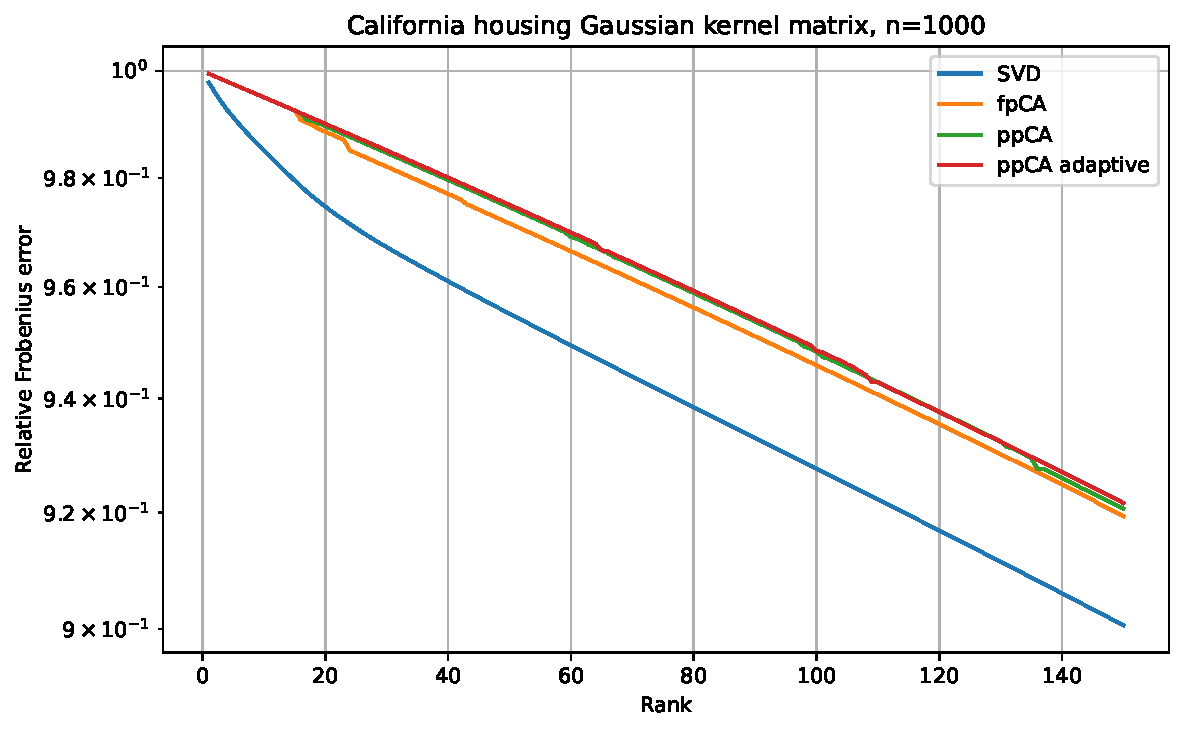
\includegraphics[width=0.85\textwidth]{plots/california_gaussian_kernel.pdf}
    \caption{Relative Frobenius error for the California housing Gaussian kernel matrix.}
    \label{fig:california_gaussian_kernel}
\end{figure}

\subsubsection*{Matrix-free experiment}

Figure~\ref{fig:matrix_free_iris_gaussian_kernel} shows the error curve for the matrix-free ppCA experiment. In this case, the approximation routine accesses the Iris Gaussian kernel only through the entry function $K(i,j)$.

\begin{figure}[h]
    \centering
    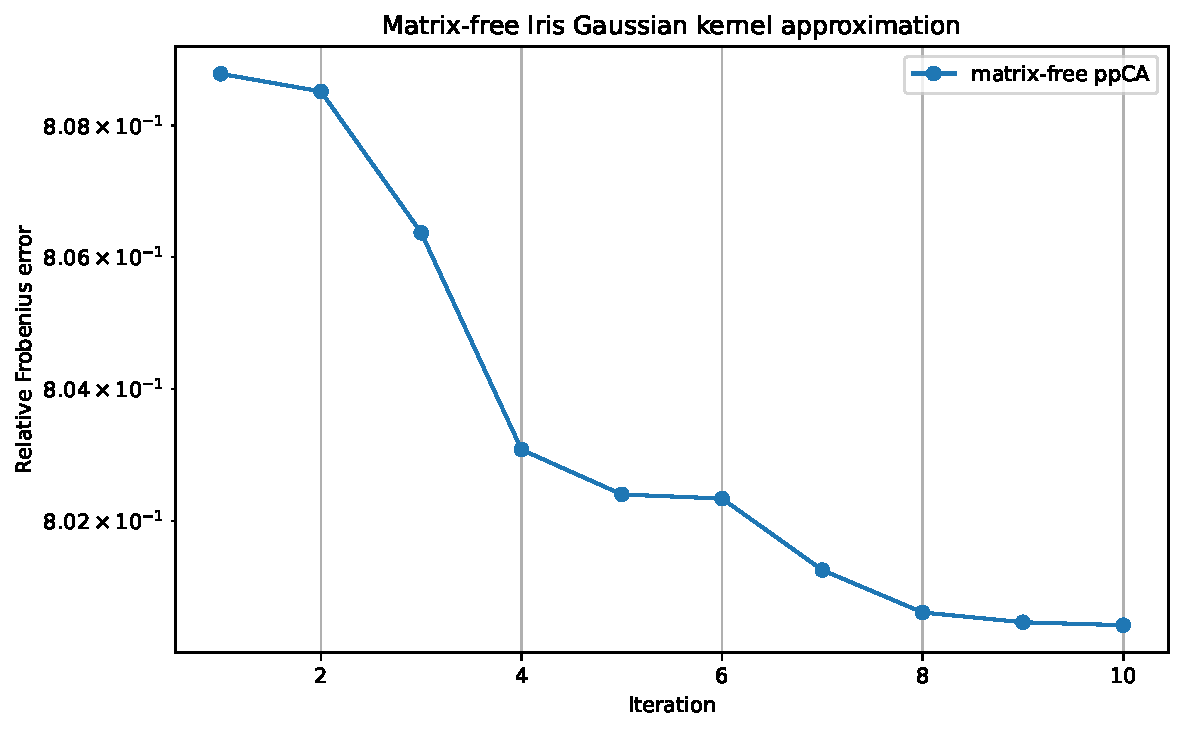
\includegraphics[width=0.85\textwidth]{plots/matrix_free_iris_gaussian_kernel.pdf}
    \caption{Relative Frobenius error for the matrix-free Iris Gaussian kernel ppCA experiment.}
    \label{fig:matrix_free_iris_gaussian_kernel}
\end{figure}

\subsection{Discussion}

The experiments illustrate that the performance of cross approximation depends strongly on the decay of the singular values and on the pivoting strategy. Full pivoting is usually more reliable because it selects the largest residual entry, but it is also more expensive and requires the full residual matrix. Partial pivoting is cheaper because it only uses one residual row and one residual column per iteration. The adaptive ppCA version avoids choosing the final rank in advance by stopping when the new rank-one update becomes small relative to the first update.

The SVD remains the optimal reference method in terms of Frobenius-norm accuracy, but it requires access to the full matrix. Cross approximation is less optimal, but it is attractive when the matrix is large, dense, or available only through individual entries.
